\documentclass[11pt]{article}
\usepackage[margin=1in]{geometry}
\usepackage{amsmath,amssymb}
\usepackage{graphicx}
\usepackage{booktabs}
\usepackage{tikz}
\usetikzlibrary{arrows.meta,positioning}
\usepackage[numbers,sort&compress]{natbib}
\usepackage[colorlinks=true,linkcolor=blue!50!black,citecolor=blue!50!black,urlcolor=blue!50!black]{hyperref}
\usepackage{microtype}

\title{\textbf{Percolation: Concepts, Universality, and Its Place in\\ Contemporary Biophysics}}
\author{Review notes}
\date{October 2026}

\begin{document}
\maketitle

\begin{abstract}
Percolation theory describes how global connectivity emerges abruptly when local, random links are added to a system. Despite its deceptively simple definition, it yields a genuine continuous phase transition with universal critical exponents, fractal clusters, and anomalous transport. In this article we first introduce the basic models (site, bond and continuum percolation), the order parameter, the scaling theory near the threshold, and the important distinction between \emph{connectivity} and \emph{rigidity} percolation. We then ask whether percolation is an active concept in present-day biophysics. The answer is clearly yes: percolation is now a central ingredient in the theory of biomolecular condensates (``phase separation coupled to percolation''), in the mechanics of cytoskeletal and extracellular fibre networks, in the solid--fluid transitions of embryonic tissues, in living neuronal networks, in diffusion through crowded membranes, and in the propagation of excitation waves and epidemics. We close with a discussion of the limits of the analogy---activity, non-equilibrium driving, and finite size---and of open questions.
\end{abstract}

\section{Introduction}

Imagine pouring water onto a porous stone. Whether the water reaches the bottom depends not on the average porosity alone but on whether the open pores form a \emph{connected path} through the whole stone. This question, posed by Broadbent and Hammersley in 1957 \cite{Broadbent1957}, gave the field its name: \emph{percolation}. In its idealised form one considers a lattice whose sites (or bonds) are independently ``open'' with probability $p$ and asks whether an infinite connected cluster of open elements exists. For small $p$ only finite clusters exist; above a sharply defined threshold $p_c$ an infinite (system-spanning) cluster appears with probability one.

Percolation is perhaps the simplest model with a non-trivial phase transition: there is no Hamiltonian, no temperature, and no interaction energy---only geometry and probability. Yet the transition at $p_c$ shares all hallmarks of thermal critical phenomena: diverging correlation length, power-law cluster statistics, scale invariance, and universality \cite{StaufferAharony,Christensen2005}. For this reason percolation has become a paradigm for connectivity transitions in fields as varied as porous media, conducting composites, gelation, forest fires, network robustness, and epidemics \cite{Sahimi1994,Newman2002,Callaway2000}.

This article has two goals. Section~\ref{sec:theory} explains what percolation is, at the level needed to read the biophysical literature. Section~\ref{sec:bio} then surveys whether, and how, contemporary biophysics uses the concept. Section~\ref{sec:discussion} discusses the conceptual caveats and open problems.

\section{What is percolation?}\label{sec:theory}

\subsection{Site, bond and continuum percolation}

In \emph{site percolation} each vertex of a lattice is occupied independently with probability $p$; neighbouring occupied sites belong to the same cluster. In \emph{bond percolation} all sites are present but each edge is open with probability $p$. In \emph{continuum percolation} objects (discs, spheres, rods) are placed at random positions in space and are connected whenever they overlap; the control parameter is then a density or volume fraction. Continuum models are often the most natural for biological systems, where filaments, proteins or cells are not arranged on a lattice.

Figure~\ref{fig:site} shows site percolation on a $120\times120$ square lattice. Below the threshold [panel (a)] the largest cluster (red) is small and the occupied sites form many isolated islands. At $p\approx p_c$ [panel (b)] the largest cluster is a ramified, tenuous object that just barely spans the system. Above $p_c$ [panel (c)] it dominates the lattice.

\begin{figure}[t]
\centering
\includegraphics[width=\textwidth]{fig_site_percolation.pdf}
\caption{Site percolation on the square lattice. (a--c) Occupied sites (grey) with the largest cluster highlighted (red), below, near and above $p_c\simeq0.5927$. (d) Fraction of sites in the largest cluster, $P_\infty$, for three linear system sizes $L$ (averages over independent realisations). As $L$ grows the curve sharpens toward a singular onset at $p_c$ (dashed line).}
\label{fig:site}
\end{figure}

\subsection{The threshold}

The percolation threshold $p_c$ is non-universal: it depends on the lattice and on whether sites or bonds are diluted (Table~\ref{tab:pc}). Only a handful of thresholds are known exactly, notably $p_c=1/2$ for bond percolation on the square lattice \cite{Kesten1980} and site percolation on the triangular lattice; most others are obtained numerically with very high precision, for example using the Newman--Ziff algorithm \cite{NewmanZiff2000}. On a tree-like (Bethe) lattice where each node has $z$ neighbours, the threshold follows from a simple branching argument: a path continues if, on average, at least one of the $z-1$ outgoing branches is open, giving
\begin{equation}
p_c^{\text{Bethe}}=\frac{1}{z-1}.
\label{eq:bethe}
\end{equation}
This is exactly the mean-field (Flory--Stockmayer) theory of polymer gelation \cite{Flory1941,Stockmayer1943}, a fact that will reappear in the biomolecular context. On random networks with degree distribution $P(k)$, the analogous criterion becomes $\langle k^2\rangle/\langle k\rangle=2$ (the Molloy--Reed criterion), which explains why heavy-tailed networks are extremely robust to random failure \cite{Callaway2000}.

\begin{table}[h]
\centering
\caption{Representative percolation thresholds.}
\label{tab:pc}
\begin{tabular}{lcc}
\toprule
Lattice & site $p_c$ & bond $p_c$\\
\midrule
Square (2D) & $0.592746\ldots$ & $1/2$ (exact)\\
Triangular (2D) & $1/2$ (exact) & $2\sin(\pi/18)\approx0.3473$ (exact)\\
Honeycomb (2D) & $0.6970\ldots$ & $1-2\sin(\pi/18)\approx0.6527$ (exact)\\
Simple cubic (3D) & $0.3116\ldots$ & $0.2488\ldots$\\
Bethe lattice, coordination $z$ & $1/(z-1)$ & $1/(z-1)$\\
\bottomrule
\end{tabular}
\end{table}

\subsection{Order parameter, cluster statistics and scaling}

The natural order parameter is the probability $P_\infty(p)$ that a randomly chosen site belongs to the infinite cluster. It vanishes for $p<p_c$ and grows continuously above it [Fig.~\ref{fig:site}(d)]. Near the threshold, observables obey power laws:
\begin{align}
P_\infty &\sim (p-p_c)^{\beta}, & \xi &\sim |p-p_c|^{-\nu}, & \chi=\langle s\rangle &\sim |p-p_c|^{-\gamma},
\end{align}
where $\xi$ is the correlation length (the typical radius of finite clusters) and $\chi$ is the mean size of finite clusters, which plays the role of a susceptibility. The cluster size distribution---the number of clusters of $s$ sites per lattice site---takes the scaling form
\begin{equation}
n_s(p)\simeq s^{-\tau}\, f\!\left[(p-p_c)\,s^{\sigma}\right],
\label{eq:ns}
\end{equation}
so that exactly at $p_c$ the cluster sizes are distributed as a pure power law, $n_s\sim s^{-\tau}$. The incipient infinite cluster at $p_c$ is a fractal of dimension $D_f=d-\beta/\nu$: its mass inside a box of size $R$ grows as $M(R)\sim R^{D_f}$.

\paragraph{Universality.} The exponents depend only on the spatial dimension (and on the range of connections), not on the lattice or on site vs.\ bond dilution. In two dimensions they are known exactly (Table~\ref{tab:exp}); above the upper critical dimension $d_c=6$ they take mean-field values. This universality is precisely what makes percolation attractive for biology: a measured exponent can, in principle, diagnose a connectivity transition without detailed knowledge of the underlying molecular interactions.

\begin{table}[h]
\centering
\caption{Critical exponents of ordinary (connectivity) percolation.}
\label{tab:exp}
\begin{tabular}{lccc}
\toprule
Exponent & $d=2$ (exact) & $d=3$ (numerical) & mean field ($d\ge6$)\\
\midrule
$\beta$ & $5/36$ & $\approx0.42$ & 1\\
$\nu$ & $4/3$ & $\approx0.88$ & $1/2$\\
$\gamma$ & $43/18$ & $\approx1.80$ & 1\\
$\tau$ & $187/91$ & $\approx2.19$ & $5/2$\\
$D_f$ & $91/48$ & $\approx2.52$ & 4\\
\bottomrule
\end{tabular}
\end{table}

\paragraph{Finite-size scaling.} In a finite system of linear size $L$ the transition is rounded, and the threshold shifts by an amount $\sim L^{-1/\nu}$. Observables collapse onto universal curves when plotted as functions of $(p-p_c)L^{1/\nu}$, e.g.\ $P_\infty=L^{-\beta/\nu}\,\tilde{P}\!\left[(p-p_c)L^{1/\nu}\right]$. This is essential in biology, where a tissue may contain only $10^2$--$10^4$ cells, and the ``transition'' is necessarily a smooth crossover.

\subsection{Transport on percolating clusters}

Connectivity does not imply efficient transport. Near $p_c$ the spanning cluster is dominated by dead ends and narrow ``red'' bonds, so the macroscopic conductivity of a random resistor network vanishes as $\Sigma\sim(p-p_c)^{t}$ with $t\approx1.3$ in 2D and $\approx2.0$ in 3D \cite{StaufferAharony}. A random walker confined to the incipient cluster diffuses anomalously, $\langle r^2(t)\rangle\sim t^{2/d_w}$ with walk dimension $d_w>2$. These results underpin much of the biophysical literature on anomalous diffusion in crowded environments (Sec.~\ref{sec:membrane}).

\subsection{Rigidity percolation}

Connectivity is not the same as mechanical stability. A network of central-force springs in $d$ dimensions can sustain stress only if it has enough constraints to remove all floppy modes. Maxwell's counting argument shows that a network of $N$ nodes with mean coordination $z$ becomes rigid when the number of constraints $Nz/2$ exceeds the number of degrees of freedom $Nd$, i.e.\ at the \emph{isostatic point}
\begin{equation}
z_c=2d .
\label{eq:maxwell}
\end{equation}
\emph{Rigidity percolation} asks when a rigid cluster first spans the system as bonds are randomly added \cite{FengSen1984,JacobsThorpe1995}. It occurs at a higher bond density than connectivity percolation (for the 2D triangular lattice, $p_r\approx0.66$ vs.\ $p_c\approx0.35$) and belongs to a different universality class. Bending stiffness of semiflexible filaments, internal stress, or active forces can stabilise networks below the Maxwell point, producing a rich ``critical'' mechanical regime \cite{Broedersz2011,Sharma2016}. This distinction---\emph{connected but floppy} versus \emph{connected and rigid}---is central for cells and tissues.

\subsection{Variants}

Many generalisations exist: \emph{directed percolation} (connections only forward in time, the universality class of absorbing-state transitions such as epidemic extinction); \emph{correlated percolation} (occupancy correlated in space); \emph{explosive} and \emph{bootstrap} percolation (abrupt or cooperative activation rules); and percolation on complex networks \cite{Callaway2000}. Several of these appear naturally when biological systems are not well described by independent random occupation.

\section{Is percolation discussed in contemporary biophysics?}\label{sec:bio}

Yes---and increasingly so. The concept appears at every scale, from multivalent proteins to tissues and populations. Table~\ref{tab:bio} summarises the main areas discussed below.

\begin{table}[t]
\centering
\small
\caption{Where percolation appears in biophysics.}
\label{tab:bio}
\begin{tabular}{p{3.1cm}p{3.4cm}p{3.2cm}p{3.6cm}}
\toprule
System & ``Sites/bonds'' & Control parameter & Type of percolation\\
\midrule
Biomolecular condensates & stickers / reversible bonds & concentration, valence, salt & connectivity (gelation), coupled to phase separation\\
Actomyosin \& fibre networks & filaments / crosslinks & crosslinker density & connectivity and rigidity\\
Embryonic tissue & cells / adhesive contacts & cell connectivity $\langle k\rangle$ & rigidity\\
Neuronal cultures & neurons / synapses & synaptic strength & bond (graph) percolation\\
Membranes & lipids, proteins / obstacles & area fraction of obstacles & site/continuum; anomalous diffusion\\
Excitable tissue, epidemics & cells or hosts / transmission & fraction of coupled cells, $R_0$ & bond percolation, directed percolation\\
\bottomrule
\end{tabular}
\end{table}

\subsection{Biomolecular condensates: phase separation coupled to percolation}

The most active current use of percolation in biophysics concerns \emph{biomolecular condensates}---membraneless compartments such as nucleoli, stress granules and P granules. Early work described them as liquid--liquid phase separation (LLPS), a density transition. A widely adopted framework, developed in particular by Pappu, Mittag and colleagues, instead treats condensate-forming proteins and RNAs as \emph{associative polymers} built from ``stickers'' (adhesive motifs) and ``spacers'' \cite{Choi2020}. Stickers form reversible physical crosslinks; when enough crosslinks form, a system-spanning network appears. This is a percolation (gelation) transition, whose mean-field description is the Flory--Stockmayer theory and Eq.~\eqref{eq:bethe}.

In this picture, condensates generally form via \emph{phase separation coupled to percolation} (PSCP): a density transition (phase separation, threshold $c_{\text{sat}}$) and a networking transition (percolation, threshold $c_{\text{perc}}$) act synergistically \cite{MittagPappu2022}. When $c_{\text{sat}}<c_{\text{perc}}$, phase separation concentrates molecules into a dense phase whose concentration exceeds $c_{\text{perc}}$, so that the dense phase is a percolated network (Fig.~\ref{fig:pscp}). The resulting condensates are \emph{viscoelastic network fluids} rather than simple liquids, with sequence-specific internal network structure and time-dependent rheology \cite{MittagPappu2022}.

\begin{figure}[t]
\centering
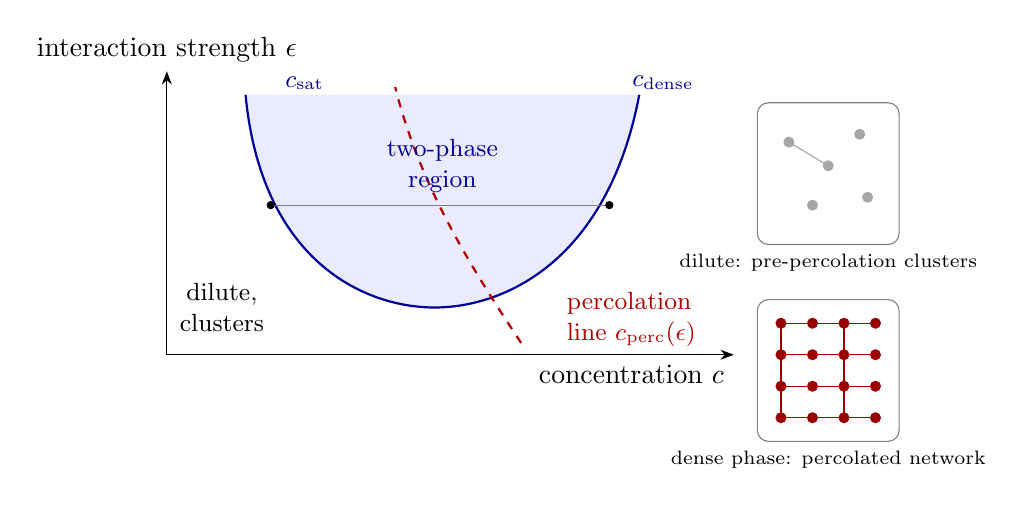
\begin{tikzpicture}[scale=1.0, >=Stealth]
 % axes
 \draw[->] (0,0) -- (7.2,0) node[below left] {concentration $c$};
 \draw[->] (0,0) -- (0,3.6) node[above] {interaction strength $\epsilon$};
 % binodal
 \fill[blue!8] (1.0,3.3) .. controls (1.2,1.2) and (2.5,0.6) .. (3.4,0.6)
        .. controls (4.3,0.6) and (5.6,1.2) .. (6.0,3.3) -- cycle;
 \draw[thick,blue!60!black] (1.0,3.3) .. controls (1.2,1.2) and (2.5,0.6) .. (3.4,0.6)
        .. controls (4.3,0.6) and (5.6,1.2) .. (6.0,3.3);
 % percolation line
 \draw[thick,dashed,red!70!black] (4.5,0.15) .. controls (3.8,1.2) and (3.2,2.2) .. (2.9,3.4);
 \node[blue!60!black,align=center,font=\small] at (3.5,2.4) {two-phase\\ region};
 \node[font=\small,align=center] at (0.7,0.6) {dilute,\\ clusters};
 \node[red!70!black,font=\small,align=left] at (5.9,0.45) {percolation\\ line $c_{\text{perc}}(\epsilon)$};
 \node[blue!60!black,font=\small] at (1.75,3.45) {$c_{\text{sat}}$};
 \node[blue!60!black,font=\small] at (6.3,3.45) {$c_{\text{dense}}$};
 % tie line
 \draw[thin,gray] (1.32,1.9) -- (5.62,1.9);
 \fill (1.32,1.9) circle (1.5pt); \fill (5.62,1.9) circle (1.5pt);
 % schematic insets
 \begin{scope}[shift={(8.4,2.3)}]
   \draw[rounded corners,gray] (-0.9,-0.9) rectangle (0.9,0.9);
   \foreach \x/\y in {-0.5/0.4,0.4/0.5,-0.2/-0.4,0.5/-0.3,0.0/0.1}{
     \fill[gray!70] (\x,\y) circle (2pt);}
   \draw[gray!70] (-0.5,0.4)--(0.0,0.1);
   \node[font=\scriptsize,below] at (0,-0.9) {dilute: pre-percolation clusters};
 \end{scope}
 \begin{scope}[shift={(8.4,-0.2)}]
   \draw[rounded corners,gray] (-0.9,-0.9) rectangle (0.9,0.9);
   \foreach \x in {-0.6,-0.2,0.2,0.6}{\foreach \y in {-0.6,-0.2,0.2,0.6}{
     \fill[red!60!black] (\x,\y) circle (2pt);}}
   \foreach \x in {-0.6,-0.2,0.2}{\foreach \y in {-0.6,-0.2,0.2,0.6}{
     \draw[red!60!black] (\x,\y)--(\x+0.4,\y);}}
   \foreach \x in {-0.6,0.2}{\foreach \y in {-0.6,-0.2,0.2}{
     \draw[red!60!black] (\x,\y)--(\x,\y+0.4);}}
   \node[font=\scriptsize,below] at (0,-0.9) {dense phase: percolated network};
 \end{scope}
\end{tikzpicture}
\caption{Schematic of phase separation coupled to percolation (PSCP) for associative biopolymers, after the framework of Refs.~\cite{Choi2020,MittagPappu2022}. Inside the coexistence region (shaded) a dilute phase at $c_{\text{sat}}$ coexists with a dense phase at $c_{\text{dense}}$. When the percolation line (dashed) lies between them, the dense phase is a system-spanning network while the dilute phase contains finite clusters whose size distribution is governed by percolation statistics.}
\label{fig:pscp}
\end{figure}

PSCP makes concrete, testable predictions that pure LLPS does not. Most notably, percolation statistics imply a broad distribution of \emph{pre-percolation clusters} already in subsaturated solutions ($c<c_{\text{sat}}$). Kar \emph{et al.} reported exactly such heterogeneous nano- and mesoscale clusters for phase-separating RNA-binding proteins in subsaturated solutions \cite{Kar2022}, and subsequent work has examined how solution conditions reshape these clusters even when the driving forces for phase separation are unchanged. Percolation also offers a natural language for \emph{ageing} of condensates (progressive network hardening), for the role of valence and linker length, and for the coexistence of liquid-like and gel-like behaviour. The framework is now standard enough to be taught in dedicated summer schools on the physical principles of condensates, alongside LLPS and polymer collapse.

It is worth stressing what percolation does \emph{not} do here: in the thermodynamic limit, gelation of reversible bonds without phase separation does not by itself produce interfaces or surface tension. It is the coupling to the density transition that yields finite droplets with interfaces; percolation controls their internal connectivity and material properties.

\subsection{Cytoskeletal and extracellular fibre networks}

The cytoskeleton is a network of filaments (actin, microtubules, intermediate filaments) linked by crosslinking proteins and driven by molecular motors. Two percolation questions arise: (i) when does the network become connected enough to transmit motor-generated forces over cellular length scales, and (ii) when does it become mechanically rigid?

For the first question, Alvarado \emph{et al.} reconstituted actin networks with tunable crosslink (fascin) density and myosin activity \cite{Alvarado2013}. They found that motors break the network into disjoint contracting clusters, and that the crossover from local to global contraction closely resembles a connectivity percolation transition; strikingly, motor activity drives networks over a broad range of initial connectivities toward a \emph{critically connected} state, with power-law cluster size distributions. Bueno \emph{et al.} generalised Flory--Stockmayer kinetic theory to actomyosin networks with different actin-binding proteins (e.g.\ $\alpha$-actinin, Arp2/3), estimating the crosslinker concentrations required for connectivity and for rigidity percolation and emphasising the difference between the two thresholds \cite{Bueno2022}. Analogous percolation-based arguments have been applied to microtubule--kinesin systems, where connectivity of bundles controls whether forces remain local or propagate globally.

For the second question, fibre networks such as collagen and fibrin gels in the extracellular matrix are typically \emph{sub-isostatic}: their mean connectivity lies between 3 and 4, well below the Maxwell threshold $z_c=6$ in 3D [Eq.~\eqref{eq:maxwell}]. They are nevertheless rigid because of filament bending and, under load, because applied strain stiffens them. Broedersz \emph{et al.} showed that bending rigidity governs a critical regime near isostaticity \cite{Broedersz2011}, and Sharma \emph{et al.} showed that the nonlinear stiffening of collagen networks is controlled by a strain-driven rigidity transition with critical scaling \cite{Sharma2016}. Rigidity percolation has thus become a standard lens for cell and tissue mechanics.

\subsection{Tissue mechanics and embryonic development}

At the multicellular scale, tissues can behave as solids or as fluids. Vertex and Voronoi models predict a rigidity transition controlled by cell shape rather than density \cite{Bi2015}. A particularly clear demonstration of percolation \emph{in vivo} came from Petridou \emph{et al.} \cite{Petridou2021}, who studied the zebrafish blastoderm during early development. Treating cells as nodes and adhesive cell--cell contacts as bonds, they showed that rigidity percolation theory predicts a material phase transition from local cell connectivity: a small reduction in adhesion-dependent connectivity below a critical value triggers tissue fluidization, with viscosity dropping by about an order of magnitude within minutes. They quantitatively predicted and experimentally verified hallmarks of a genuine transition---power-law exponents and discontinuities in macroscopic observables---and showed that the uniformity of the transition across the tissue depends on meta-synchronous cell divisions that randomise changes in connectivity, as percolation theory assumes \cite{Petridou2021}. Follow-up work has extended this framework to link rigidity transitions to germ-layer formation and cell-fate decisions.

\subsection{Neuronal networks}

In living neural cultures, Breskin \emph{et al.} used the network's response to electrical stimulation while gradually weakening synaptic coupling with a chemical antagonist \cite{Breskin2006}. The size of the largest connected (``giant'') component shrank continuously to zero at a critical coupling strength, mapping the problem onto bond percolation on a graph and allowing inference of the network's degree distribution. Percolation ideas continue to be used to analyse functional connectivity, the robustness of neural circuits to damage, and the onset of global bursts in developing cultures.

\subsection{Membranes and crowded environments}\label{sec:membrane}

Biological membranes are crowded with proteins, cytoskeletal fences and lipid domains. When the area fraction of immobile obstacles approaches the percolation threshold, the accessible region becomes a fractal cluster and lateral diffusion becomes anomalous, $\langle r^2\rangle\sim t^{\alpha}$ with $\alpha<1$ \cite{Saxton1994}. Monte Carlo studies of obstructed diffusion on lattices established this connection early on, and it remains a standard reference point for interpreting single-particle tracking data. Percolation of ordered lipid domains (``rafts'') or of protein clusters has likewise been invoked to explain abrupt changes in membrane connectivity and signalling. The cytoplasm itself, with its high macromolecular volume fraction, has been modelled as a medium near a percolation-like glass or gel transition.

\subsection{Excitable media and wave propagation}

Excitation waves---action potentials in heart tissue, calcium waves, or cAMP waves in aggregating \emph{Dictyostelium} amoebae---propagate only if excitable elements are sufficiently connected. When a fraction of cells is non-excitable or uncoupled (e.g.\ fibrotic cardiac tissue), wave propagation becomes a percolation problem. Alonso and B\"ar showed in a discrete model of cardiac tissue that reentrant waves (a precursor to arrhythmia) are most likely near the percolation threshold of the excitable cells \cite{AlonsoBar2013}. For systems such as \emph{Dictyostelium}, the emergence of collective cAMP signalling depends on cell density \cite{Gregor2010}; while this onset is usually discussed as a dynamical (quorum-like) transition rather than a geometric one, percolation provides a useful complementary framework whenever relay requires spatial contact or short-range coupling between excitable cells, and heterogeneity in excitability is spatially random.

\subsection{Epidemics and populations}

The final size of an SIR epidemic maps exactly onto bond percolation, with transmissibility playing the role of $p$ \cite{Grassberger1983,Newman2002}. The epidemic threshold is the percolation threshold of the contact network, and the expected outbreak size is the size of the giant component. Real-time dynamics near the threshold belong to the directed percolation class. These mappings are used routinely in theoretical epidemiology and in microbial ecology (e.g.\ spread of phage or of cooperative traits in spatially structured colonies).

\section{Discussion: strengths, limits and open questions}\label{sec:discussion}

Percolation is attractive in biophysics because it links \emph{local} quantities that can be measured or genetically manipulated---number of stickers on a protein, crosslinker concentration, adhesive contacts per cell, synaptic strength---to \emph{global} emergent properties such as gelation, force transmission, tissue rigidity, or signal propagation. Its universality suggests that a few exponents might classify very different biological transitions.

Several caveats, however, are important:
\begin{enumerate}
\item \textbf{Finite size.} Cells contain a limited number of molecules and embryos a limited number of cells. Transitions are rounded, and critical exponents can be extracted only over narrow ranges. Finite-size scaling must be used explicitly, and claims of criticality require care.
\item \textbf{Correlations.} Classical percolation assumes independent random occupation. Biological bonds are correlated (cooperative binding, spatial patterning, mechanical feedback), which can change the universality class or render the transition discontinuous.
\item \textbf{Reversibility and dynamics.} Molecular bonds in condensates and cytoskeleta form and break on time scales comparable to observation. Percolation then describes an instantaneous network; rheology depends on bond lifetimes, and ``gel'' vs.\ ``liquid'' becomes time-scale dependent.
\item \textbf{Activity.} Motors, cell divisions and ATP-driven remodelling drive systems far from equilibrium. Active networks can self-organise to criticality \cite{Alvarado2013}, but the mapping to equilibrium percolation is not guaranteed.
\item \textbf{Connectivity vs.\ function.} A connected network need not be rigid, and a rigid one need not transmit chemical signals efficiently. Choosing the right percolation variant (connectivity, rigidity, directed, bootstrap) is part of the modelling.
\end{enumerate}

Open questions include: how cells regulate proximity to percolation thresholds (e.g.\ via post-translational modifications that change valence); whether biological systems exploit critical connectivity for sensitivity and robustness; how coupled percolation transitions across scales (molecular networks within cells within tissues) interact; and how to measure network connectivity directly \emph{in vivo} with quantitative imaging.

\section{Conclusion}

Percolation theory describes the emergence of long-range connectivity from random local connections. It yields a sharp threshold, universal critical exponents, fractal clusters and anomalous transport, and it has a mechanically distinct cousin in rigidity percolation. Far from being a niche topic, percolation is now an established and actively developing concept in biophysics. It is a central ingredient in the modern theory of biomolecular condensates (PSCP), a standard framework for cytoskeletal and extracellular-matrix mechanics, a quantitatively validated explanation for tissue fluidization in the zebrafish embryo, and a long-standing tool for neuronal networks, membrane diffusion, excitable media and epidemics. The main frontier lies in extending the theory to correlated, reversible, finite and actively driven networks---the conditions that characterise living matter.

\begin{thebibliography}{99}\small
\setlength{\itemsep}{1pt}

\bibitem{Broadbent1957} S.~R. Broadbent and J.~M. Hammersley, ``Percolation processes,'' \emph{Proc. Cambridge Philos. Soc.} \textbf{53}, 629 (1957).

\bibitem{StaufferAharony} D.~Stauffer and A.~Aharony, \emph{Introduction to Percolation Theory}, 2nd ed. (Taylor \& Francis, London, 1994).

\bibitem{Christensen2005} K.~Christensen and N.~R. Moloney, \emph{Complexity and Criticality} (Imperial College Press, London, 2005).

\bibitem{Sahimi1994} M.~Sahimi, \emph{Applications of Percolation Theory} (Taylor \& Francis, London, 1994).

\bibitem{Newman2002} M.~E.~J. Newman, ``Spread of epidemic disease on networks,'' \emph{Phys. Rev. E} \textbf{66}, 016128 (2002).

\bibitem{Callaway2000} D.~S. Callaway, M.~E.~J. Newman, S.~H. Strogatz, and D.~J. Watts, ``Network robustness and fragility: percolation on random graphs,'' \emph{Phys. Rev. Lett.} \textbf{85}, 5468 (2000).

\bibitem{Kesten1980} H.~Kesten, ``The critical probability of bond percolation on the square lattice equals 1/2,'' \emph{Commun. Math. Phys.} \textbf{74}, 41 (1980).

\bibitem{NewmanZiff2000} M.~E.~J. Newman and R.~M. Ziff, ``Efficient Monte Carlo algorithm and high-precision results for percolation,'' \emph{Phys. Rev. Lett.} \textbf{85}, 4104 (2000).

\bibitem{Flory1941} P.~J. Flory, ``Molecular size distribution in three dimensional polymers. I. Gelation,'' \emph{J. Am. Chem. Soc.} \textbf{63}, 3083 (1941).

\bibitem{Stockmayer1943} W.~H. Stockmayer, ``Theory of molecular size distribution and gel formation in branched-chain polymers,'' \emph{J. Chem. Phys.} \textbf{11}, 45 (1943).

\bibitem{FengSen1984} S.~Feng and P.~N. Sen, ``Percolation on elastic networks: new exponent and threshold,'' \emph{Phys. Rev. Lett.} \textbf{52}, 216 (1984).

\bibitem{JacobsThorpe1995} D.~J. Jacobs and M.~F. Thorpe, ``Generic rigidity percolation: the pebble game,'' \emph{Phys. Rev. Lett.} \textbf{75}, 4051 (1995).

\bibitem{Broedersz2011} C.~P. Broedersz, X.~Mao, T.~C. Lubensky, and F.~C. MacKintosh, ``Criticality and isostaticity in fibre networks,'' \emph{Nat. Phys.} \textbf{7}, 983 (2011).

\bibitem{Sharma2016} A.~Sharma, A.~J. Licup, K.~A. Jansen, R.~Rens, M.~Sheinman, G.~H. Koenderink, and F.~C. MacKintosh, ``Strain-controlled criticality governs the nonlinear mechanics of fibre networks,'' \emph{Nat. Phys.} \textbf{12}, 584 (2016).

\bibitem{Choi2020} J.-M. Choi, A.~S. Holehouse, and R.~V. Pappu, ``Physical principles underlying the complex biology of intracellular phase transitions,'' \emph{Annu. Rev. Biophys.} \textbf{49}, 107 (2020).

\bibitem{MittagPappu2022} T.~Mittag and R.~V. Pappu, ``A conceptual framework for understanding phase separation and addressing open questions and challenges,'' \emph{Mol. Cell} \textbf{82}, 2201 (2022).

\bibitem{Kar2022} M.~Kar \emph{et al.}, ``Phase-separating RNA-binding proteins form heterogeneous distributions of clusters in subsaturated solutions,'' \emph{Proc. Natl. Acad. Sci. USA} \textbf{119}, e2202222119 (2022).

\bibitem{Alvarado2013} J.~Alvarado, M.~Sheinman, A.~Sharma, F.~C. MacKintosh, and G.~H. Koenderink, ``Molecular motors robustly drive active gels to a critically connected state,'' \emph{Nat. Phys.} \textbf{9}, 591 (2013).

\bibitem{Bueno2022} C.~Bueno, J.~Liman, N.~P. Schafer, M.~S. Cheung, and P.~G. Wolynes, ``A generalized Flory--Stockmayer kinetic theory of connectivity percolation and rigidity percolation of cytoskeletal networks,'' \emph{PLoS Comput. Biol.} \textbf{18}, e1010105 (2022).

\bibitem{Bi2015} D.~Bi, J.~H. Lopez, J.~M. Schwarz, and M.~L. Manning, ``A density-independent rigidity transition in biological tissues,'' \emph{Nat. Phys.} \textbf{11}, 1074 (2015).

\bibitem{Petridou2021} N.~I. Petridou, B.~Corominas-Murtra, C.-P. Heisenberg, and E.~Hannezo, ``Rigidity percolation uncovers a structural basis for embryonic tissue phase transitions,'' \emph{Cell} \textbf{184}, 1914 (2021).

\bibitem{Breskin2006} I.~Breskin, J.~Soriano, E.~Moses, and T.~Tlusty, ``Percolation in living neural networks,'' \emph{Phys. Rev. Lett.} \textbf{97}, 188102 (2006).

\bibitem{Saxton1994} M.~J. Saxton, ``Anomalous diffusion due to obstacles: a Monte Carlo study,'' \emph{Biophys. J.} \textbf{66}, 394 (1994).

\bibitem{AlonsoBar2013} S.~Alonso and M.~B\"ar, ``Reentry near the percolation threshold in a heterogeneous discrete model for cardiac tissue,'' \emph{Phys. Rev. Lett.} \textbf{110}, 158101 (2013).

\bibitem{Gregor2010} T.~Gregor, K.~Fujimoto, N.~Masaki, and S.~Sawai, ``The onset of collective behavior in social amoebae,'' \emph{Science} \textbf{328}, 1021 (2010).

\bibitem{Grassberger1983} P.~Grassberger, ``On the critical behavior of the general epidemic process and dynamical percolation,'' \emph{Math. Biosci.} \textbf{63}, 157 (1983).

\end{thebibliography}
\end{document}
